\documentclass{beamer}
\usepackage[latin1]{inputenc}
\usepackage{graphicx}
\usetheme{Rochester}

\title{Julia Sets}
\author{Taran Dike}\institute{University of Washington}

\begin{document}

\begin{frame}
\titlepage
\end{frame}

\begin{center}

\begin{frame}
Julia Set:
A set of complex numbers that do not converge to any limit when a given mapping is repeatedly applied to them. In some cases the result is a connected fractal set.
\end{frame}

\begin{frame}
First, a bit of background.
\end{frame}

\begin{frame}
Gaston Julia, a French Mathematician, published a paper in 1918 concerning iterationsions of a rational function.  Despite initial popularity, the fame quickly faded...
\end{frame}

\begin{frame}
until Benoit Mandelbrot discovered the Mandelbrot set in 1979 with the assistance of modern computers.  This allowed him to create images of the sets.  Now fractals are immensely popular.
\end{frame}

\begin{frame}
A Julia Set is an example of a set with chaotic behavior in Complex Dynamics.  It is iterated multiple times over some $c$ value to obtain the image.  Any small change to $c$ has a large effect.  Hence the chaotic behavior.
\end{frame}

\begin{frame}
This particular Sage function uses the equation $z = z^2 + c$ to generate its Julia Set images.  There are certainly other possibilities including cubic equations, exponentials, etc., but the quadratic equation is simple and quite popular.
\end{frame}

\begin{frame}
The code is written in Python.  It creates a .pgm (Portable Graymap) file, which is essentially a series of numbers corresponding to a grayscale.
\end{frame}

\begin{frame}
A very small sample of a .pgm file:
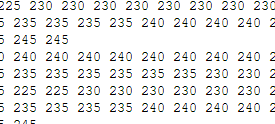
\includegraphics{JuliaPGMScreenshot}
\end{frame}

\begin{frame}
Julia Set with $c = -0.8 + 0.156i$
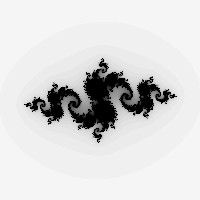
\includegraphics{Julia1}
\end{frame}

\begin{frame}
Julia Set with $c = 0.285 + 0.01i$
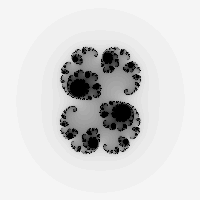
\includegraphics{Julia2}
\end{frame}

\begin{frame}
Julia Set with $c = 0.70176 - 0.3842i$
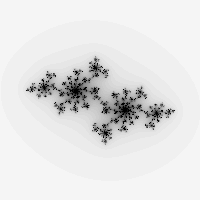
\includegraphics{Julia3}
\end{frame}

\begin{frame}
*I picked random numbers from here on out.
\end{frame}

\begin{frame}
Julia Set with $c = -0.045 + 0.764i$
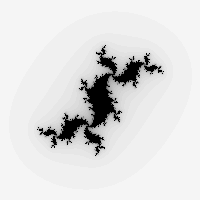
\includegraphics{Julia4}
\end{frame}

\begin{frame}
*It doesn't always result in a nice image.
\end{frame}

\begin{frame}
Julia Set with $c = 0.876 + 0.259i$
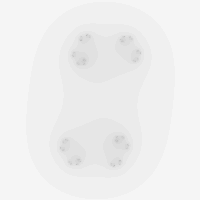
\includegraphics{Julia5}
\end{frame}

\begin{frame}
Julia Set with $c = -0.378 - 0.594i$
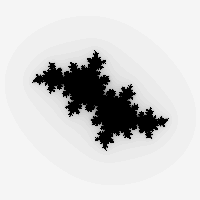
\includegraphics{Julia6}
\end{frame}

\begin{frame}
These next two have very similar $c$ values.  I changed the real component by 0.05.
\end{frame}

\begin{frame}
Julia Set with $c = 0.45 - 0.57i$
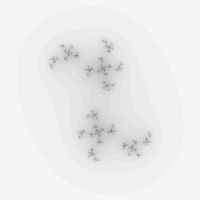
\includegraphics{Julia7}
\end{frame}

\begin{frame}
Julia Set with $c = 0.50 - 0.57i$
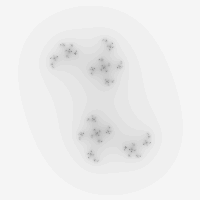
\includegraphics{Julia8}
\end{frame}

\begin{frame}
There are many different iteration methods available to plot fractals. Fractals have become quite popular as a focus of jewelry, photography, and other art.
\end{frame}

\begin{frame}
Thank You
\end{frame}

\end{center}

\end{document}
%sagemathcloud={"zoom_width":90}